\documentclass[UTF8]{ctexart}

\usepackage[body={15cm, 23cm}, top={2.5cm}]{geometry}
\usepackage{cite}
\usepackage{graphicx}
\CTEXsetup[format={\Large\bfseries}]{section}

\title{\textbf{基于移动群智感知的无线网络数据收集
       稀疏性问\\
       题研究\\
       Research on Data Sparseness of Wireless Network
       Based on Mobile\\
       Crowdsensing}}
\begin{document}
\maketitle
\section{选题依据}
\subsection{选题的背景、目的和意义}

移动群智感知(Mobile Crowd Sensing, MCS)的概念最早由Raghu K. Ganti等人提出的,
是一种利用普通的社会群众进行信息感知的数据收集技术[1],它将普通用户的移动设备作为
基本感知单元,通过移动互联网进行有意识或无意识的协作,形成移动群智感知网络,实现
感知任务分发与感知数据收集,然后在云端对这些数据汇集及融合,最终用于以人为中心服
务的数据交付[2]。

群智感知网络成在为新型的重要感知手段,可利用普适的移动感知设备完成仅依靠个体很难
实现的大规模、复杂的社会感知任务。目前,移动群智感知的相关应用涉及到各个方面,如
环境监测[4][5]、社交网络[8]、健康[9]、交通[6][7]等方面。此外,移动群智感知
技术也应用与无线环境数据的收集,比如收集Wi-Fi数据[10][11][12],收集蜂窝网络数据
[13][14]。在使用移动群智感知的方法进行数据感知的过程中为了更加全面的获取到目标感
知区域的环境信息,需要大量的感知节点最大化的覆盖整个感知区域[3]。在实际应用移动
群智感知技术进行数据收集的时候,由于客观条件的限制会出现参与感知的节点数量少,感知到
的数据规模小的情况。一方面,由于在感知任务的过程当中,用户需要消耗自己移动终端的电能、
数据流量,除此之外还可能会暴露用户的移动轨迹、位置信心和通话记录等相关的隐私信息,
所以用户不愿意无偿的参加感知任务,造成参与感知节点数量少[15][16]。虽然针对参与感知
用户少,感知数据稀疏且质量不高的问题,通过设计适当的激励机制来鼓励用户参与到感知任务
中去[17][18],但是参与感知的用户少,数据稀疏的问题仍然出现[19]。另一方面,由于数据
的稀疏性,数据规模小,种类少,所以无法根据稀疏的数据全面的了解目标感知区域的无线环境
的分布情况。

为了解决由于数据的稀疏性带来的无法全面而准确的还原目标感知区域的环境信息的问题,
本研究提出了一种适合解决利用群智感知收集无线网络环境数据稀疏性问题方案。对于参与感知的
用户数量少,造成感知数据稀疏的问题,在本研究中将利用参与感知用户的移动特点来分配任务,
招募感知用户,最大化的收集无线网络环境数据。对于稀疏数据无法准确的刻画目标感知区域
无限网络环境性的问题,将利用无线网络环境数据的时空相关性推测出缺少的数据,然后通过
感知的数据和推测的数据还原出目标感知区域的无线网络环境的信息。

本研究解决了利用移动群智感知收集无线网络环境中由于数据稀疏无法准确刻画目标感知区域的
无线网络环境行信息的问题,因此本研究具有价值。

\subsection{国内外研究现状}
\subsubsection{移动群智感知概述}

随着智能设备的进一步普及,群智感知的发展也愈加迅速,在市价生活的应用也越来越广泛,
现阶段的移动群智感知应用大致可以分成三类:环境、公共设施和社会[5]。移动群智感知
的理论研究也涵盖了感知过程的各个阶段。利用移动群智感知的收集数据的过程大体可以分成
四个阶段,感知任务的生成、任务的分发、任务的执行与数据整合。感知任务的生成就是确定
使用移动群智感知的方法来收集哪些数据,例如收集任务参与者的GPS记录或者不同地理位置
的噪声分贝。在任务的分发阶段,Xiao提出了一种新的任务分发的方法,将任务在移动社交
网络中分别以离线和在线的方式进行分发[20]。在感知任务执行阶段使用piggyback的方法能够
有效的节省设备的消耗的能量[21]。最后一个阶段的数据传输和整个阶段,将现有的路由协议
进行升级,提出了性的适合机会传输的新的路由协议[22]。

\subsubsection{移动群智感知中数据稀疏性研究现状}

移动群智感知技术大量应用于无线环境数据的收集。Shi在刻画
建筑中Wi-Fi信息时,保证了足够大的覆盖比例和数据量,通过
感知的数据刻画了建筑中无线网络的分布及使用状况[23]。此外,在使用移动群智感知收集蜂窝网络
数据的过程中,Deterding也提出了使用人类移动规律来收集更多的蜂窝网络数据,刻画了一个
CBD区域内LTE信号的分布情况[24]。

解决使用移动群智感知方法收集无线网络数据收集的稀疏性而不能准确的刻画无线网络环境的问题
可以通过两个步骤解决。首先,进行稀疏感知,利用已有参与感知的感知节点最大化的收集与无线
网络相关的数据;然后,利用已有的数据和根据无线网络数据的时空特性来推测缺失的数据刻画目
标感知区域的无线网络分布情况。

\subparagraph{\textbf{(1) 稀疏感知与人移动规律}}

稀疏感知首先由Leye明确在群智感知的框架下提出,稀疏感知是在移动群智感知中使用较少的感知
节点完成整个目标感知区域的感知任务,进而减少数据的冗余度和感知系统的开销[25]。此外在Li
的文章中相应的提到了使用车联网进行感知的时候会出现数据缺失的问题,并提出了使用相应的激
励机制来诱导车辆进行感知以解决数据缺失的问题[26]。文献[27][28]介绍了和移动群智感知中
的稀疏感知相似的应用于车联网的压缩感知的感知方式。稀疏感知是在移动群智感知的框架下提出
的非常新的感知方式,还没有将其应用到无线网络数据收集的应用当中,并且上述的压缩感知使用
的是车联网的情景,并不完全适合人携带移动终端进行感知的情景。

在移动群智感知中,人作为感知节点,参与感知的用户携带移动终端进行任务感知,所以我们可以
充分利用用户移动规律来感知环境的信息。人类的移动轨迹具有一定的规律可循,
并且可以根据人的历史移动轨迹可以推测到一个人在移动过程中的下一个目的地,并且预测的正确
率可达到93\%[29][30]。我们可以根据用户移动规律来感知更多无线环境数据。在文献[31]中Sara
利用用户的移动规律符合截断的列维飞行模型来选择用户注册参与到感知任务中来,建立概率模型
使用用户最大化的覆盖用目标感知区域。在Shenggong的文中,城市感知系统进行任务发布的时候
待参与感知的用户上报自己的行程(时间、目的地和路线),然后由感知系统根据用户的移动规律
来对待参与感知的用户进行筛选[32]。

\subparagraph{\textbf{(2) 稀疏数据的推测与还原}}

由于参与感知的用户数量较少,所以收集到的数据规模小,数据呈现出稀疏性。要对目标感知区域
的无线网络的分布状况进行较为准确的刻画,需要的数据量要大,所以要根据已经感知到的数据对
缺失的数据进行推测还原,根据感知的数据和推测的数据刻画出无线网络分布的状况。在[33]的文献
中介绍,在车联网进行感知的时候针对数据的缺失可以使用插值算法、主成分分析、矩阵和张量
补全的方法进行结合感知数据的时空相关性来实现缺失数据较为精确的估计。Mendez介绍了插值算法
在参与式感知系统中的数据恢复中的应用,分别使用马尔科夫随机场和和克里金插值算法进行较为准
确的预测车联网系统中参与式感知缺失的数据[34]。在[35]中介绍的压缩感知应用于车联网,利用
主程序分析的方法较为精确的预测了交通路况。虽然,上述关于数据预测的算法能够精确的预测车
联网感知中缺失的数据,但是尚未应用于利用群智感知的方法收集无线网络数据。

\subsection{当前存在的问题}
\subparagraph{(1) 将人类移动规律应用于稀疏感知过程以收集更多的数据。}

通过将参与用户的移动
规律应用到无线网络环境的感知过程中可以感知到更多的数据。由于用户的移动规律在较短时间
内呈现出一定的随机性,所以如何得到用户的移动规律以及将用户的移动规律应用于群感知感知的
哪个过程,如何将用户的移动规律与移动群智感知结合起来是值得研究的问题。

\subparagraph{(2) 利用稀疏的感知数据推测出缺失的数据并准确的刻画无线网络环境。}

由于感知数据的稀疏性,所以无法根据已有的数据准确地刻画目标感知区域的无线网络环境。要
根据现有感知到的数据结合感知数据的时空特性来推测出缺失的部分数据,但是目前应用于
恢复稀疏数据的算法尚未应用与群智感知中,要选择一种适合无线网络数据时空特性的算法
用于缺失数据的预测与恢复。

\section{研究的目标和主要研究内容}
\subsection{研究目标}

本研究的主要目标是解决在使用移动群智感知的方法进行无线网络数据感知的过程中由于参与感知的用户
规模小造成的感知数据稀疏,数据质量下降,进而无法通过已有的数据进行准确的刻画目标感知区域的
无线网络环境数据的问题。

\subsection{主要研究内容}

本研究的重点研究的是利用移动群智感知的方式对无线网络数据收集机制。由于的参与感知任务的用户
数量少,造成目标感知区域的数据不完整,数据质量下降的问题。因此,为了收集高质量的无线网络数
据,并准确的刻画目标感知区域的无线网络环境信息,本研究中首先研究如何通过少量的感知节点结合
人的移动规律感知更多感知数据;其次,如何通过稀疏的感知数据推测得到目标感知区域的无线网络数
据。具体研究内容如下:

\subparagraph{(1) 移动群智感知结合人类移动规律进行数据感知。}

在少量的用户参与到无线网络数据的感知时,可以将人的移动规律结合到感知任务中,因为在使用移
动群智感知的方法进行数据感知时,感知终端是由人携带进行任务感知的。通过某段时间人的移动规律,
可以得到感知节点在感知区域的移动规律,那么感知节点可以在这段时间感知到不同地方的无线网络
数据指标。由与参与感知的用户规模小,但是由于人携带的感知设备处于移动的状态中,充分利
用人类的移动规律可以使少量的感知节点获得较多感知数据。因此,在研究少量用户参与无线网络
数据的感知过程中可以将人的移动规律结合到群智感知的过程中。

\subparagraph{(2) 利用已感知数据预测目标感知区域内缺失的数据。}

在利用了人类的移动规律进行最大化无线网络数据感知之后,由于数据的稀疏性,没有感知到完整的
目标感知区域无线网络数据,不能够刻画整个目标感知区域的无线网络数据的分布情况。虽然数据是
不完整的,但是由于无线网络数据其自身所具有的时空特性,我们可以通过对已有的感知数据进行预
测,进而获得整个感知区域的无线网络数据,解决由于参与用户少带来的感知数据稀疏性。

\subparagraph{(3) 仿真验证。}

对本课题提出的任务分配算法进行仿真,分析、验证所提任务分配机制的有效性。

\section{拟解决的关键问题及其研究方法}
\subsection{拟解决的关键问题}
\subparagraph{(1) 移动群智感知结合人类移动规律进行数据感知。}

在少量的用户参与到无线网络数据的感知时,可以将人的移动规律结合到感知任务中,因为在使用移
动群智感知的方法进行数据感知时,感知终端是由人携带进行任务感知的。通过某段时间人的移动规律,
可以得到感知节点在感知区域的移动规律,那么感知节点可以在这段时间感知到不同地方的无线网络
数据指标。由与参与感知的用户规模小,但是由于人携带的感知设备处于移动的状态中,充分利
用人类的移动规律可以使少量的感知节点获得较多感知数据。因此,在研究少量用户参与无线网络
数据的感知过程中可以将人的移动规律结合到群智感知的过程中。

\subparagraph{(2) 利用已感知数据预测目标感知区域内缺失的数据。}

在利用了人类的移动规律进行最大化无线网络数据感知之后,由于数据的稀疏性,没有感知到完整的
目标感知区域无线网络数据,不能够刻画整个目标感知区域的无线网络数据的分布情况。虽然数据是
不完整的,但是由于无线网络数据其自身所具有的时空特性,我们可以通过对已有的感知数据进行预
测,进而获得整个感知区域的无线网络数据,解决由于参与用户少带来的感知数据稀疏性。

\subsection{采取的研究方法}
\subparagraph{(1) 利用参与者的移动规律进行感知参与者的招募和任务的分发。}

利用人类的移动规律进行感知任务参与者的招募和任务分发时,通过这种办法可以实现较少参与者
收集更多的数据并且可以最大化的覆盖到目标感知区域,进而提高数据质量。如图1中所示,首先
感知任务的设计者发布目标感知区域以及需要进行感知的时间段,当然也包括相应的回报,需要感
知的网络网络的相应的指标数据。如果用户对发布的无线网络环境数据的感知任务感兴趣, 那么
用户(例如用户$u_1$,$u_2$,$u_3$,$u_4$)会在感知任务开始之前提交他们的移动轨迹的
相关信息,包括他们出发地点、目的地点、花费的时间和出行路线。感知系统通过对用户提交的移动
轨迹的相关信息来判断参与用户是否适合参与到感知任务的中,在所有用户中选择部分适合参与感知
任务的用户(例如用户$u_1$,$u_2$)。通过这种方式我们可以根据用户的移动规律选择出参与用户
并且可以提高感知用户对感知区域的覆盖比例。

\par
\centerline{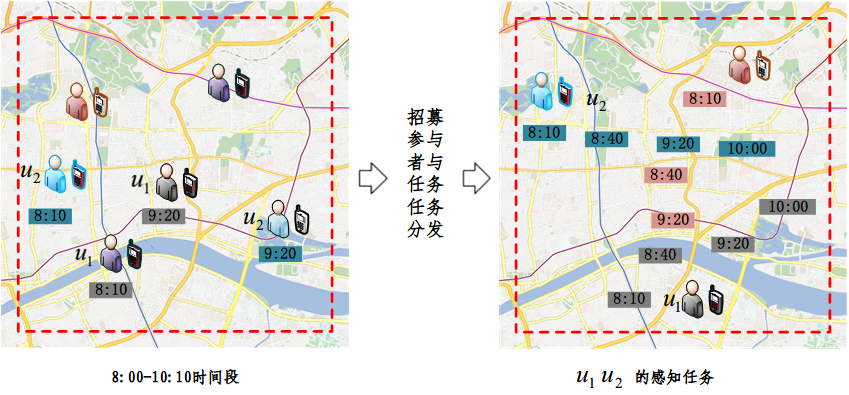
\includegraphics[width=5in]{1.png}}
%%要居中就用centerline,这里的图片和tex 文件在一个目录下
\centerline{图1 利用人类的移动规律招募参与用户并进行任务分发}
将上面的问题通过数学的方式进行描述。

\emph{定义用户} 我们将每一个参与感知的用户用一个元组进行$u$表示,$u \leq l_s,l_e,t_s,t_e $,
其中$l_s,l_e,t_s,t_e$ 分别表示参与者的出发地点,目的地点,出发时间和到达时间。

\emph{定义感知任务} 无线网络中的感知任务(sensing task)可以表示为$s$,$s$是一个与感知
地点相关的时间段序列。例如$s=(l_1,t_1)\rightarrow(l_2,t_2)\rightarrow\cdots$,其中$l$
表示数据收集的位置,$t$表示数据收集的时间段。

\emph{定义感知数据} 通过上面的数学表达,可以定义已经感知到的数据可以用一个三维的向量来表示$V$,
那么$V(i,j,t)$表示在位置$(i,j)$的$(t)$时间段内收集到的数据。

根据上面的已经定义的用户,感知任务和感知数据,那么利用人类的移动规律最大化的收集数据可以通过
数学的表达形式描述为下面表达式:

\[ s.t.=
\begin{cases}
\Sigma_u, \quad u,r<B \\
max V, \quad V
\end{cases}
\]


\subparagraph{(2) 使用插值算法根据已感知数据对确实数据进行预测}
由于无线网络环境数据的环境中无线网络指标的分布随着地理位置的不同而发生变换,所以拟使用
插值算法进行数据预测。使用插值算法根据已有的数据对缺失的数据进行估计预测拟采用的插值算法
为克里金(kriging)插值算法,克里金算法常用于地质环境的预测中,因此拟使用克里金算法用于
环境中无线网络数据预测。

克里金法假定采样点之间的距离或方向可以反映可用于说明表面变化的空间相关性。克里金法工具可
将数学函数与指定数量的点或指定半径内的所有点进行拟合以确定每个位置的输出值。克里金法是一
个多步过程;它包括数据的探索性统计分析、变异函数建模 和创建表面,还包括研究方差表面。

克里金法可对周围的测量值进行加权以得出未测量位置的预测,这两种插值器的常用公式均由数据
的加权总和组成。

\begin{thebibliography}{99}
  \bibitem{1} Luo, Tie, H. P. Tan, and L. Xia. Profit-maximizing incentive
  for participatory sensing. IEEE INFOCOM IEEE, 2014:127-135.
  (pp.127-135). IEEE.
  \bibitem{2} Wu Y, Zeng JR, Peng H, Chen H, Li CP. Survey on incentive
  mechanisms for crowd sensing. Ruan Jian Xue Bao.2016.
  \bibitem{3} Liu C, Software S O. Experimental Incentive Mechanisms for
  Crowd Sensing[J]. Zte Technology Journal, 2015.
  \bibitem{4} Dutta P, Aoki P M, Kumar N, et al. Common Sense: participatory
  urban sensing using a network of handheld air quality monitors[C]
  International Conference on Embedded Networked Sensor Systems, SENSYS 2009,
  Berkeley, California, Usa, November. 2009:349-350.
  \bibitem{5} Rana R K, Chou C T, Kanhere S S, et al. Ear-phone: an
  end-to-end participatory urban noise mapping system[C] ACM/IEEE
  International Conference on Information Processing in Sensor Networks.
  ACM, 2010:105-116.
  \bibitem{6} Thiagarajan A, Ravindranath L, Lacurts K, et al. VTrack:
  accurate, energy-aware road traffic delay estimation using mobile phones
  [C] 2009:85-98.
  \bibitem{7} Mathur S, Jin T, Kasturirangan N, et al. ParkNet: Drive-by
  Sensing of Road-Side Parking Statistics[C] 2010:123-136.
  \bibitem{8}	Giuseppe C., Andrea C., Antonio C., et al. The Participant
  Mobile Crowd Sensing Living Lab: The Testbed for Smart Cities.[J]. IEEE
  Communications Magazine ,2014,52(10):78-85
  \bibitem{9} Eisenman S B, Miluzzo E, Lane N D, et al. BikeNet: A mobile
  sensing system for cyclist experience mapping[J]. ACM Transactions on
  Sensor Networks, 2009, 6(1):2939-2965.
  \bibitem{10} Farshad, Arsham, Mahesh K. Marina, and Francisco Garcia.
  Urban WiFi characterization via mobile crowdsensing. 2014 IEEE Network
  Operations and Management Symposium (NOMS). IEEE, 2014.
  \bibitem{11} Chon, Yohan, et al. Sensing WiFi packets in the air:
  practicality and implications in urban mobility monitoring. Proceedings
  of the 2014 ACM International Joint Conference on Pervasive and Ubiquitous
  Computing. ACM, 2014.
  \bibitem{12} Guo, Weisi, and Siyi Wang. Mobile crowd-sensing wireless
  activity with measured interference power. IEEE Wireless Communications
  Letters 2.5 (2013): 539-542.
  \bibitem{13} Foremski, Paweł, et al. Energy-efficient crowdsensing of human
  mobility and signal levels in cellular networks. Sensors 15.9 (2015):
  22060-22088.
  \bibitem{14} Ding, Guoru, et al. Cellular-base-station-assisted
  device-to-device communications in TV white space. IEEE Journal on Selected
  Areas in Communications 34.1 (2016): 107-121.
  \bibitem{15} Liu Y, Guo B, Wang Y, et al. TaskMe: multi-task allocation
  in mobile crowd sensing[J].2016
  \bibitem{16} Lee J S, Hoh B. Sell your experiences: a market mechanism
  based incentive for participatory sensing[C] IEEE International Conference
  on Pervasive Computing and Communications. IEEE, 2010:60-68.
  \bibitem{17} Zhang D, Wang L, Xiong H, et al. 4W1H in mobile crowd
  sensing[J]. IEEE Communications Magazine, 2014, 52(8):42-48.
  \bibitem{18} Rachuri K K, Mascolo C, Musolesi M, et al. SociableSense:
  Exploring the Trade-offs of Adaptive Sampling and Computation Offloading for
  Social Sensing[C] 2011:73-84.
  \bibitem{19}	Xiao M, Wu J, Huang L, et al. Multi-task assignment for
  crowdsensing in mobile social networks[C]. 2015.
  \bibitem{20} Xiao M, Wu J, Huang L, et al. Multi-task assignment for
  crowdsensing in mobile social networks[C] Computer Communications. IEEE,
  2015:2227-2235.
  \bibitem{21}	Lane N D, Chon Y, Zhou L, et al. Piggyback CrowdSensing (PCS):
  energy efficient crowdsourcing of mobile sensor data by exploiting smartphone
  app opportunities[C]. 2013:1-14.
  \bibitem{22} Verma A, Srivastava A. Integrated Routing Protocol for
  Opportunistic Networks[J]. International Journal of Advanced Computer Science
  \& Applications, 2011, 2(3).
  \bibitem{23} Shi J, Meng L, Striegel A, et al. A walk on the client side:
  Monitoring  enterprise Wifi networks using smartphone channel scans[C]
  IEEE INFOCOM 2016 - IEEE Conference on Computer Communications. IEEE, 2016:1-9.
  \bibitem{24} Xiong H, Zhang D, Wang L, et al. EMC 3 : Energy-efficient data
  transfer in mobile crowdsensing under full coverage constraint[J]. IEEE
  Transactions on Mobile Computing, 2015, 14(7):1355-1368.
  \bibitem{25} Wang L, Zhang D, Wang Y, et al. Sparse mobile crowdsensing:
  challenges and opportunities[J]. IEEE Communications Magazine, 2016, 54(7):
  161-167.
  \bibitem{26} Jinglin L I, Yuan Q, Yang F. Crowd Sensing and Service in
  Internet of Vehicles[J]. Zte Technology Journal, 2015.
  \bibitem{27} Zhu Y, Li Z, Zhu H, et al. A Compressive Sensing Approach to
  Urban Traffic Estimation with Probe Vehicles[J]. IEEE Transactions on Mobile
  Computing, 2013, 12(11):2289-2302.
  \bibitem{28} Zhi Li, Yanmin Zhu, Hongzi Zhu, et al. Compressive Sensing
  Approach to Urban Traffic Sensing[M]. IEEE, 2011.
  \bibitem{29} Song C, Barabási A L. Limits of Predictability in Human Mobility[J].
  Science, 2010, 327(5968):1018-1021.
  \bibitem{30} Song C, Koren T, Wang P, et al. Modelling the scaling properties
  of human mobility[J]. Nature Physics, 2010, 6(10):818-823.
  \bibitem{31} Hachem S, Pathak A, Issarny V. Probabilistic registration for
  large-scale mobile participatory sensing[C] IEEE International Conference
  on Pervasive Computing and Communications. 2013:132-140.
  \bibitem{32} Ji S, Zheng Y, Li T. Urban sensing based on human mobility[C]
  ACM International Joint Conference. 2016:1040-1051.
  \bibitem{33} Jinglin L I, Yuan Q, Yang F. Crowd Sensing and Service in Internet
  of Vehicles[J]. Zte Technology Journal, 2015.
  \bibitem{34} Mendez D, Labrador M, Ramachandran K. Data interpolation for
  participatory sensing systems[J]. Pervasive \& Mobile Computing, 2013, 9(1):
  132-148.
  \bibitem{35} Zhi Li, Yanmin Zhu, Hongzi Zhu, et al. Compressive Sensing
  Approach to Urban Traffic Sensing[M]. IEEE, 2011.
\end{thebibliography}
\end{document}
